\section{Additional Results}
\label{sec:app_results}

\para{The headline edit.}
\Tabref{tab:headline} gives the results for \edit{2+2}{5} alone.

\begin{table}[h]
\centering
\caption{The edit \edit{2+2}{5} on \llama. The closest any weight edit came to ``nothing else changed'' was one flipped probe out of 990 (\ftmlp at layer 20, one run).}
\label{tab:headline}
\small
\begin{tabular}{@{}lrcccccc@{}}
\toprule
Arm & Runs & Para. & Comp.\ ent. & T/F & Flips, all & Same old ans. & KL \\
\midrule
\icl instruction & 1 & 1.00 & 0.29 & 1.00 & 0.089 & 0.18 & 0.369 \\
\gate L20, largest zero-leak $\epsilon$ & 1 & 0.76 & 0.00 & 0.00 & {\bf 0.000} & {\bf 0.00} & {\bf 0.000} \\
\gate L20, $\epsilon$ from anchors & 1 & 0.88 & 0.00 & 0.00 & 0.005 & 0.03 & 0.038 \\
\rome, L5 & 1 & 0.74 & 0.00 & 0.20 & 0.852 & 0.70 & 7.362 \\
\ftmlp, L20 & 1 & 0.68 & 0.00 & 0.00 & 0.001 & 0.03 & 0.006 \\
\loraexact & 3 & 0.97 & 0.05 & 0.00 & 0.545 & 0.83 & 1.805 \\
\loraexact, lr/10 & 3 & 0.91 & 0.00 & 0.00 & 0.031 & 0.32 & 0.148 \\
\lorakl & 3 & 0.90 & 0.00 & 0.00 & 0.006 & 0.12 & 0.051 \\
\loraparakl & 3 & 0.91 & 0.00 & 0.00 & 0.008 & 0.12 & 0.041 \\
\loradeep & 3 & 0.90 & 0.48 & 0.00 & 0.003 & 0.03 & 0.037 \\
\sdf, 120 steps & 2 & 1.00 & 0.29 & 0.35 & 0.071 & 0.06 & 0.310 \\
\bottomrule
\end{tabular}
\end{table}

\para{Change by probe category.}
\Figref{fig:heatmap} shows the fraction of probes whose answer changed in each category.

\begin{figure}[h]
    \centering
    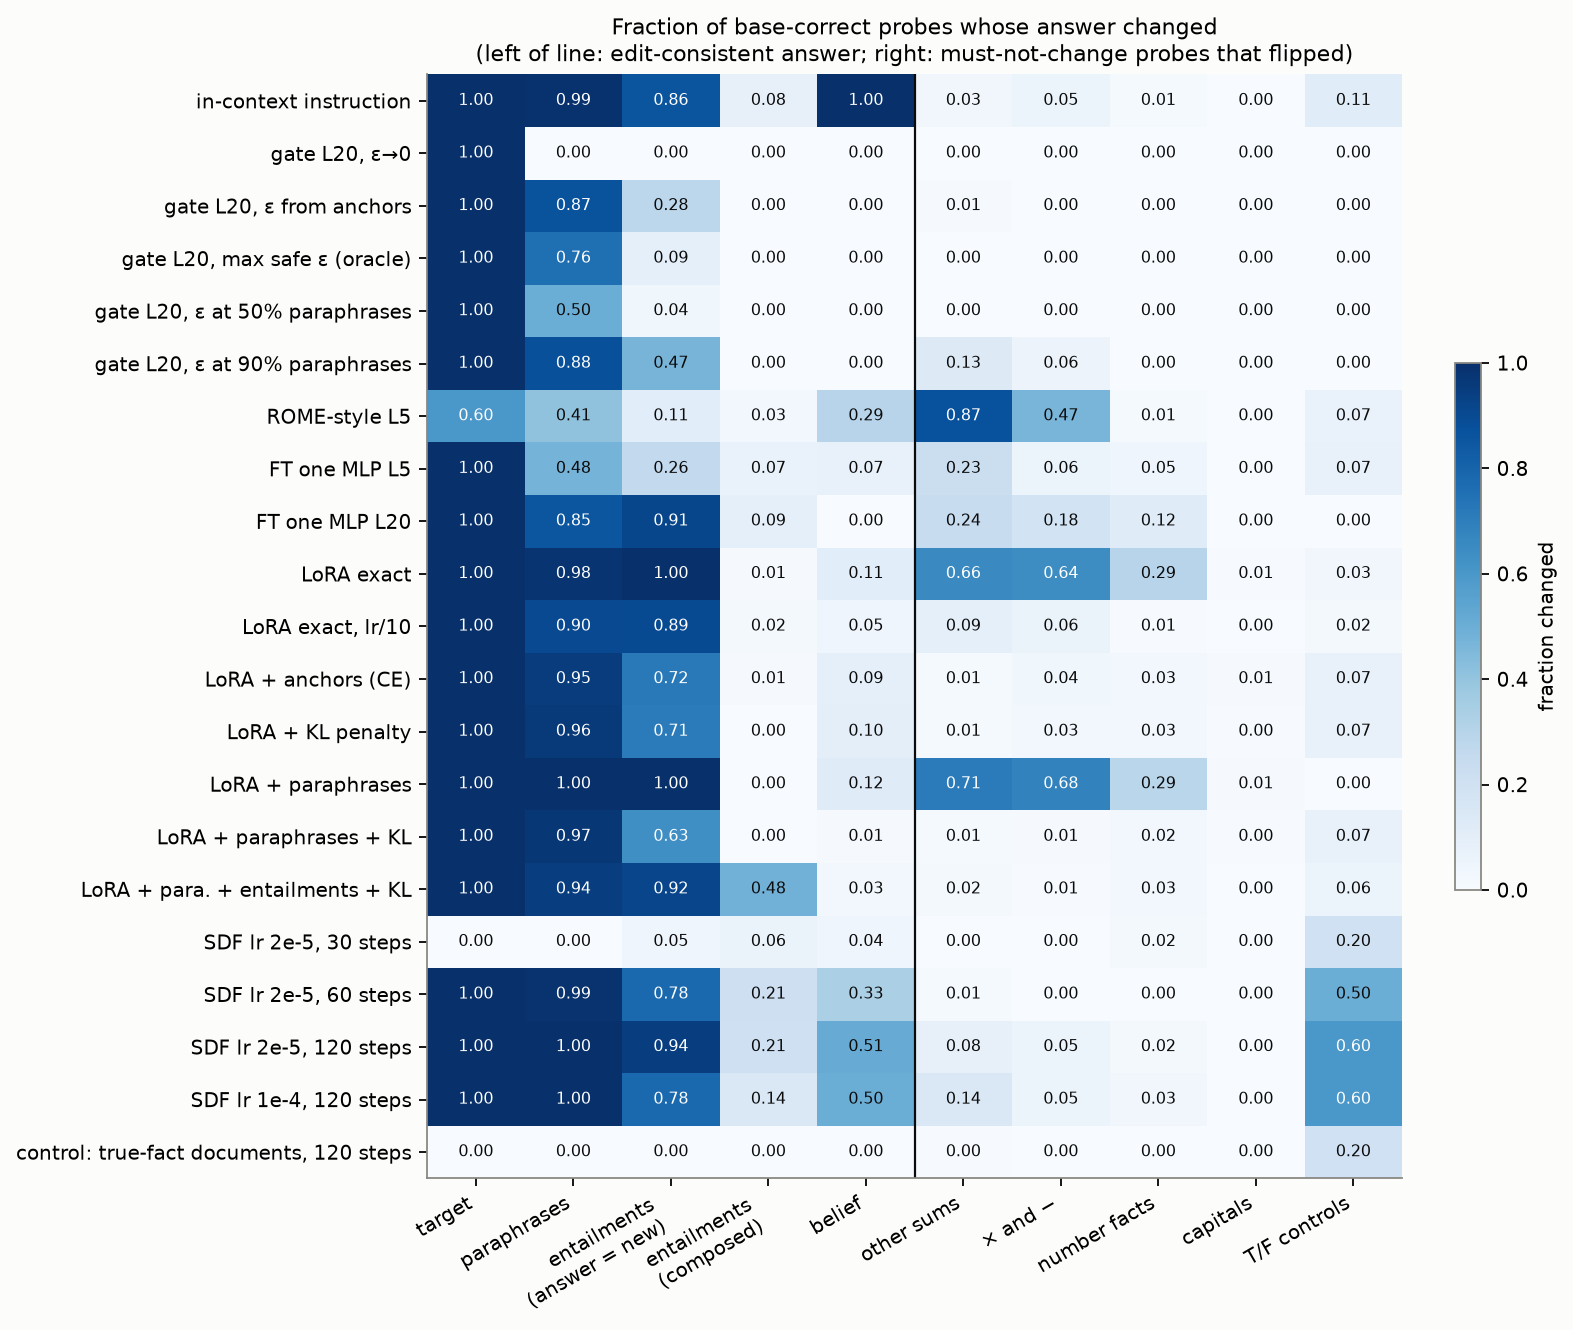
\includegraphics[width=0.8\linewidth]{figures/category_heatmap.png}
    \caption{Fraction of base-correct probes whose answer changed, by category. Left of the line the change is consistent with the edit; right of it, a must-not-change probe flipped.}
    \label{fig:heatmap}
\end{figure}

\para{Layer sweep and hyper-parameter sweeps.}
\Figref{fig:layersweep} shows single-layer fine-tuning across layers, and \figref{fig:sweeps} shows the learning-rate and KL-weight sweeps.

\begin{figure}[h]
    \centering
    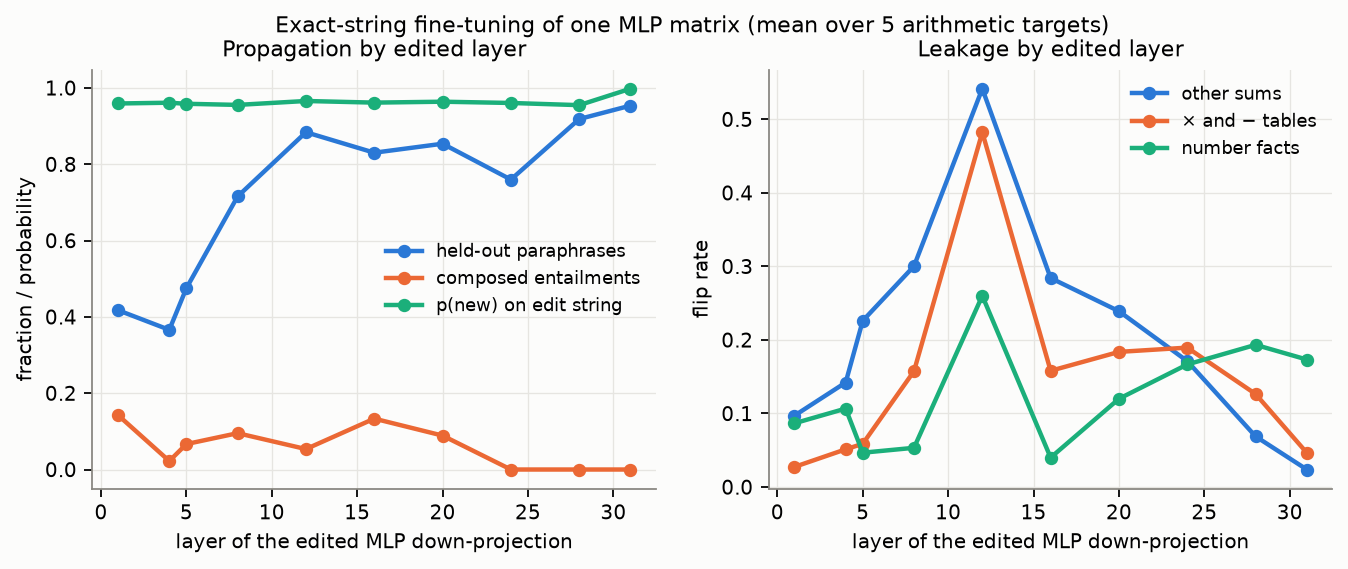
\includegraphics[width=0.85\linewidth]{figures/layer_sweep.png}
    \caption{Fine-tuning one MLP down-projection on the exact string, by layer. Paraphrase generalization rises from 0.37--0.42 at layers 1--4 to 0.76--0.95 at layers 12--31; flips on other sums peak at layer 12 (0.54) and fall to 0.02 at layer 31.}
    \label{fig:layersweep}
\end{figure}

\begin{figure}[h]
    \centering
    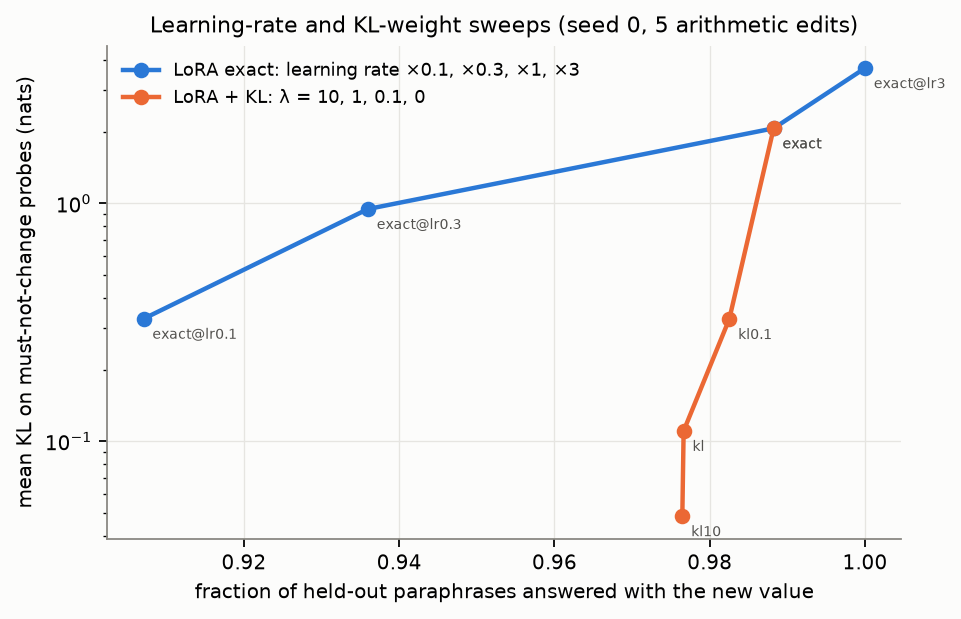
\includegraphics[width=0.6\linewidth]{figures/sweeps.png}
    \caption{Sweeps with seed 0 over five edits. Lowering the learning rate reduces leakage and paraphrase generalization together. Raising the KL weight reduces leakage about forty-fold with almost no loss of paraphrase generalization.}
    \label{fig:sweeps}
\end{figure}

\para{Unrelated behaviour.}
\Tabref{tab:drift} reports drift on unrelated distributions.
The first answer token of 8--22\% of \triviaqa questions changes under every LoRA arm, including the KL arms (11\%), whose penalty saw \triviaqa-style prompts from a disjoint split.
The base model is correct on only 51\% of these questions and many first tokens are low-confidence, so this measures sensitivity, not lost knowledge.

\begin{table}[h]
\centering
\caption{Drift on unrelated behaviour for the arithmetic edits on \llama. ``Changed'' is the fraction of prompts whose top-1 first answer token changed. \gsm is reported for two edits.}
\label{tab:drift}
\resizebox{\textwidth}{!}{%
\begin{tabular}{@{}lrccccccc@{}}
\toprule
Arm & Runs & Number facts flipped & Capitals flipped & \counterfact changed & \triviaqa changed & \wikitext KL/token & \wikitext ppl ratio & \gsm \\
\midrule
Base model & -- & -- & -- & -- & -- & -- & -- & 0.79 \\
\loraexact & 15 & 0.293 & 0.007 & 0.023 & 0.170 & 0.0019 & 1.001 & 0.81, 0.80 \\
\loraexact, lr/10 & 15 & 0.007 & 0.000 & 0.014 & 0.081 & 0.0009 & 1.000 & 0.79, 0.78 \\
\lorakl & 15 & 0.031 & 0.004 & 0.031 & 0.109 & 0.0026 & 1.002 & 0.80, 0.85 \\
\loraparakl & 15 & 0.024 & 0.004 & 0.026 & 0.113 & 0.0027 & 1.002 & 0.78, 0.80 \\
\rome, L5 & 5 & 0.013 & 0.000 & 0.017 & 0.016 & 0.0006 & 1.000 & 0.81, 0.80 \\
\icl instruction & 5 & 0.013 & 0.000 & 0.326 & 0.305 & -- & -- & 0.24, 0.32 \\
\bottomrule
\end{tabular}}
\end{table}
